\chapter{~\LaTeX~的安装}

~\LaTeX~的使用需要安装相关的软件,目前主要使用的有两种方式进行~\LaTeX~编辑:
\begin{itemize}
    \item 在线编辑器(Overleaf)
    \item 本地编辑器(VSCode+插件、TeXShop)
\end{itemize}

个人推荐使用Overleaf进行编辑,无需安装本地编译环境,同时还可以进行多人协同操作。但使用在线编辑器的缺点就是必须连接网络。

\section{Overleaf的使用}

进入到Overleaf首页:\url{https://www.overleaf.com},点击右上角Register注册新账户。登录成功后如图\ref{fig:1-overlead-home}所示,会进入到项目界面。

\begin{figure}[htb]
    \centering
    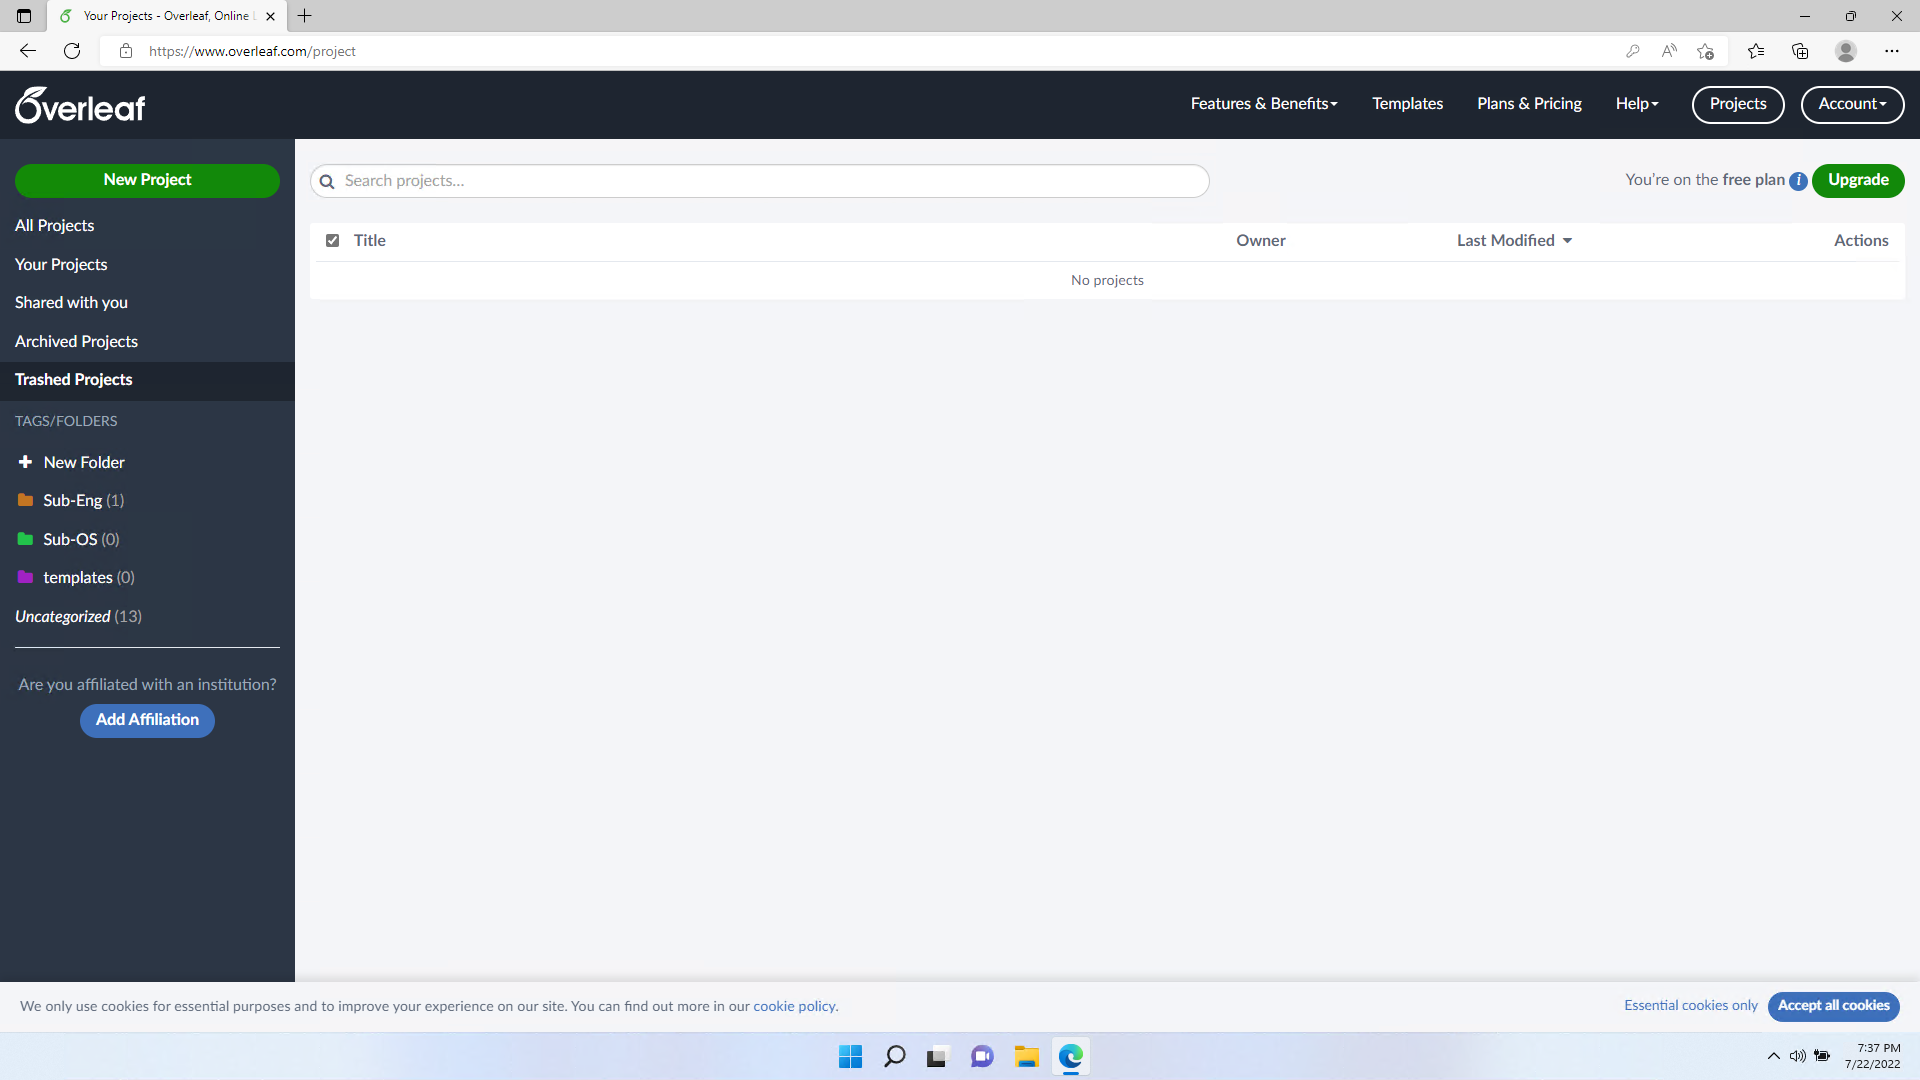
\includegraphics[width=0.9\textwidth]{figures/chapter2/overleaf-home.png}
    \caption{Overleaf项目页面}
    \label{fig:1-overlead-home}
\end{figure}

此时你需要将使用的模板下载至本地。